\section{Auswertung}
\subsection{Umrechnung in Magnetfelder}
Zu Beginn der Auswertung musste die Zeitachse des Oszilloskops in Tesla umgerechnet werden um die $B_{FW}$ zu bestimmen, welches in Gleichung \ref{tau} zu nutzten. Hierfür wurde eine gerade durch die Rampenspannung angepasst. Hierfür wurde aus dem Python Paket \verb|scipy.optimize|\cite{SciPy_Opti} das Modul \verb|curve_fit| verwendet. Für den Fit wurde die Form $f(x)=mx+b$ angenommen und an alle Werte zwischen $-1\,$V und $1\,$V als angepasst. Es wurde exakt dieser Bereich gewählt, da der echte Magnetfeld erzeugende Strom nur in diesem Bereich liegen kann und so auch die Platos vor Beginn und nach dem Ende der Rampe kategorisch ausgeschlossen werden können. Mit dieser Kurve kann nun die Messwerte der x-Achse in Tesla umgerechnet werden. Dies wurde für jede CSV Datei einzeln Durchgeführt. In Abbildung \ref{MagnetfeldAbbildung} ist ein Fit beispielhaft eingezeichnet.\par
\begin{figure}[ht]
	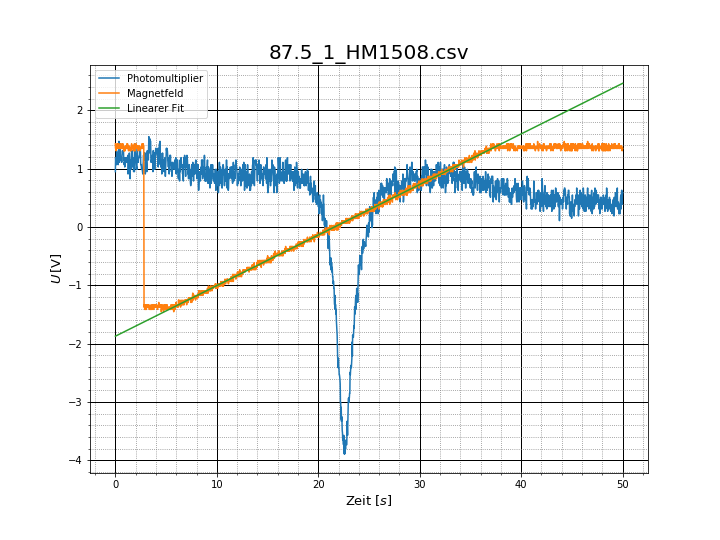
\includegraphics[scale=0.5]{Bild/Magnetfeldcali.png}
	\centering
	\caption[Magnetfeld Kalibration]{Beispiel für den Fit der Rampenspannung einer $90^\circ$ Messung. In blau die gemessenen Verlauf der Spannung des Photomultipliers. In orange die Rampenspannung und in grün der Fit.}
	\label{MagnetfeldAbbildung}
\end{figure}
\subsection{Berechnung der Lebenszeit bei $0^\circ$ und $90^\circ$}
Zur Bestimmung der Lebenszeit wurden Lorentzkurven an die Messpunkte mit der neuen x-Achse angepasst. Hierfür wurde wie zuvor \verb|curve_fit| verwendet. Die Fehler der Umrechnung des Magnetfeldes wurden nicht mitgenommen da \verb|curve_fit| keine Fehler in x-Achse zulässt. Der Fit ist diesmal in der Form:
\begin{equation}
	f(x)=\frac{a}{1+\frac{\left(x-x_0\right)^2}{\gamma^2}}+b
	\label{Lorenzfit}
\end{equation}
Der Parameter $\gamma$ ist hierbei $\frac{B_{FW}}{2}$ also die halbe Halbwertsbreite. Damit ergibt sich aus Gleichung \ref{tau}:
\begin{equation}
	\tau=\frac{\hbar}{g_J\mu_B2\gamma}
\end{equation} 
Der Fehler $\sigma_\tau$ ergibt sich durch Gaußsche Fehlerfortpflanzung mit Gleichung \ref{Fehlertau}
\begin{equation}
	\sigma_\tau=\frac{\hbar}{g_J\mu_B2\gamma^2}\sigma_\gamma
	\label{Fehlertau}
\end{equation}
Für die zwei Winkel sind Abbildung \ref{Lo0} und \ref{Lo90} Beispielhaft dargestellt.\par
\begin{figure}[ht]
	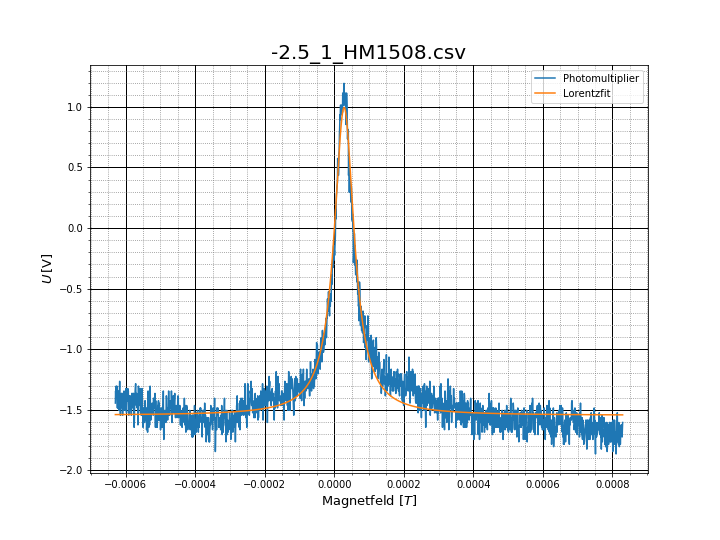
\includegraphics[scale=0.5]{Bild/GradLorenz0}
	\centering
	\caption[Fit der Lorentzkurve bei Nullgrad]{Fit der Messung bei $0^\circ$ mit dem dazugehörigen Fit als Beispiel.}
	\label{Lo0}
\end{figure}
\begin{figure}[ht]
	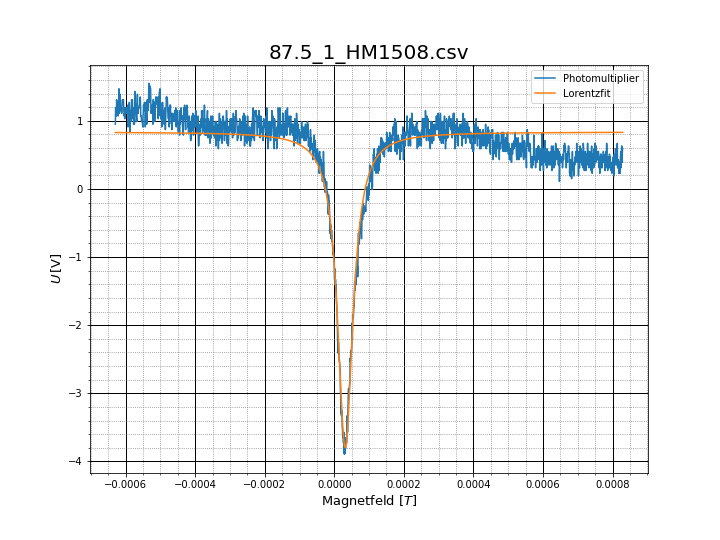
\includegraphics[scale=0.5]{Bild/90GradLorenz}
	\centering
	\caption[Fit der Lorentzkurve bei für 90Grad]{Fit der Messung bei $90^\circ$ mit dem dazugehörigen Fit als Beispiel.}
	\label{Lo90}
\end{figure}
\FloatBarrier
Zur Bestimmung des Fehlers wurde die Messung bei $0^\circ$ $15$ mal bei gleicher Temperatur von $20^\circ$ wiederholt um eine bessere Einschätzung des statistischen Fehlers auf die Lebenszeit zu bekommen (Abbildungen sind im Anhang). Als erstes wurde ein Histogramm mit den Werten von $\gamma$ (vgl. Fig. \ref{Lorenzfit}) erstellt und anschließend versucht, darüber eine Gaußkurve zu fitten um den Fehler zu bestimmen. Hierbei ergab sich die Grafik in Abbildung \ref{Fail}. Da sich hier keine schöne Gaußkurve ergab wurde alternativ die Streuung der Parameterbestimmt. Hierfür wurde die folgende Gleichung verwendet:
\begin{equation}
	\sigma_{\gamma Streuung}=\sqrt{\left(\frac{1}{n-1}\sum_{i=1}^{n}(x_i-\bar{x})^2\right)}
\end{equation}
Der hierdurch erhaltene Fehler  von $\sigma_{\gamma Streuung}=6,1\cdot10^{-7}\,$T wird von nun zu den Fehler des Parameters in allen zukünftigen Fits quadratisch addiert.
\begin{figure}[ht]
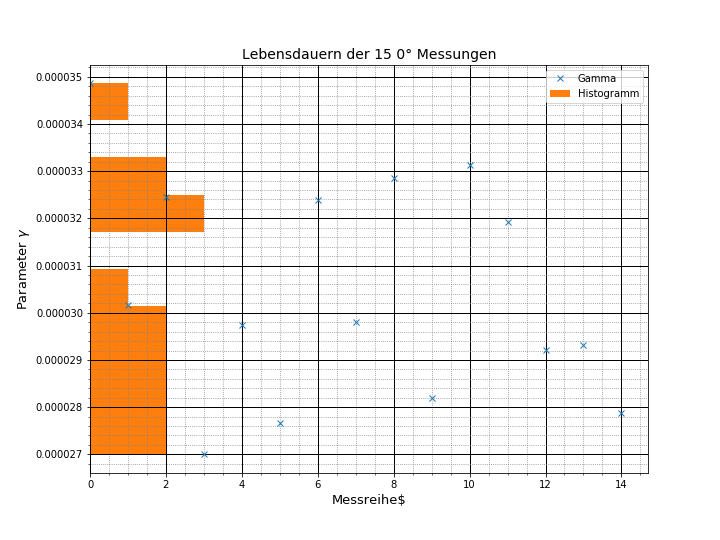
\includegraphics[scale=0.5]{Bild/gammas_hist}
\centering
\caption[Histogramm zur Bestimmung der Fehler]{Histogramm der Fit Parameter $\gamma$ von $15$ $0^\circ$ Messungen bei selber Temperatur.}
\label{Fail}
\end{figure}
\subsection{Extrapolation zur Ausschließung des Coherence Narrowing Effektes}
Die für verschiedene Temperaturen kann nun mit der Gleichung \ref{Coherence} der Druck bestimmt werden. Der Fehler des Drucks $\sigma_p$ wird mittels Gaußscher Fehlerfortpflanzung bestimmt:
\begin{equation}
\sigma_p = \frac{\partial p}{\partial T} \sigma_T
\end{equation}
Der Messfehler für die Temperatur wurde auf $0.5\,$K geschätzt.\par
Um Coherence Narrowing auszuschließen werden nun der aus der Temperatur bestimmte Druck gegen die Lebensdauer gezeichnet. Hierbei wurde wieder ein linearer Fit der Form $f(x)=mx+b$ gewählt und mit \verb|curve_fit| erstellt. Der Fehler der Lebensdauer wurde mit berücksichtigt. Mit einer Extrapolation kann man die Lebensdauer am Punkt $p=0\,$Pa also dem Parameter $b$ bestimmen. Diese ist dann die echte Lebenszeit ohne Coherence Narrowing. 
\subsubsection{Lebensdauern der Abkühlungsmessung 1}
Für die erste Abkühlungsmessung ergeben sich die nachfolgenden Werte aus den angepassten Kurven in Fig. \ref{Abk1}:
\begin{equation*}
	f(p)_{0^\circ}=(2.4 \pm 1.4)\cdot 10^{-11} \frac{\text{s}}{\text{$\mu$Pa}}\cdot p + (1.224\pm 0.022)\cdot 10^{-7} \text{s}
\end{equation*}
\begin{equation*}
	f(p)_{90^\circ}=(9.0\pm 2.6)\cdot 10^{-11} \frac{\text{s}}{\text{$\mu$Pa}}\cdot p + (1.222\pm 0.020)\cdot 10^{-7} \text{s}
\end{equation*}
Hierbei ist der y-Achsen Abschnitt jeweils die gesuchte Lebensdauer.
\begin{figure}[ht]
	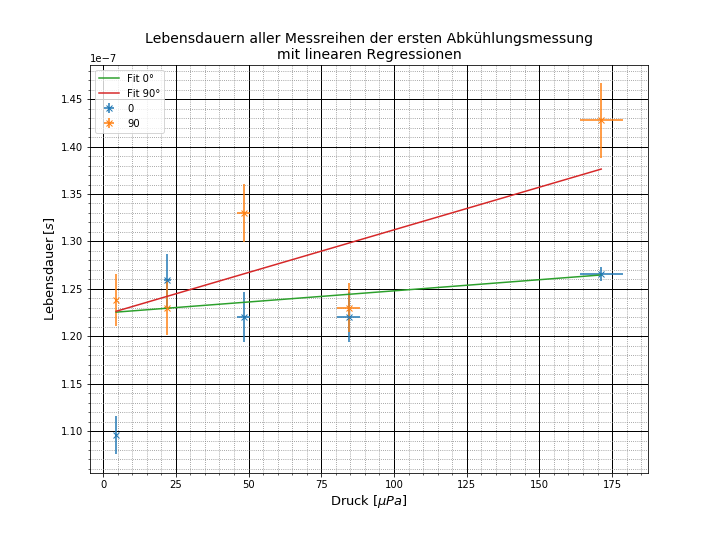
\includegraphics[scale=0.5]{Bild/Abk1}
	\centering
	\caption[Druck zu Lebensdauer Fit für Abkühlung 1]{Abkühlungsmessung der ersten Messreihe einmal für $90^\circ$ und einmal für $0^\circ$. Die Datenpunkte sind mit Fehlern für Lebensdauer und Druck aber für den Fit wurden nur die dominanteren der Lebensdauer verwendet. Der Messpunkt bei ca. $0\,\mu$Pa der 0$^\circ$ Messreihe wurde als Ausreißer nicht bei der Regression berücksichtigt.}
	\label{Abk1}
\end{figure}
\FloatBarrier
\subsubsection{Lebensdauern der Aufwärmmessung 1}
Für die Aufwärmmessung erhält man für die Angepassten Kurven (vgl. fig. \ref{Auf1}):

\begin{equation*}
f(p)_{0^\circ}=(1.4\pm 0.5)\cdot 10^{-10} \frac{\text{s}}{\text{$\mu$Pa}}\cdot p + (1.028\pm 0.013)\cdot 10^{-7} \text{s}
\end{equation*}

Hierbei ist der y-Achsen Abschnitt jeweils die gesuchte Lebensdauer.
\begin{figure}[ht]
	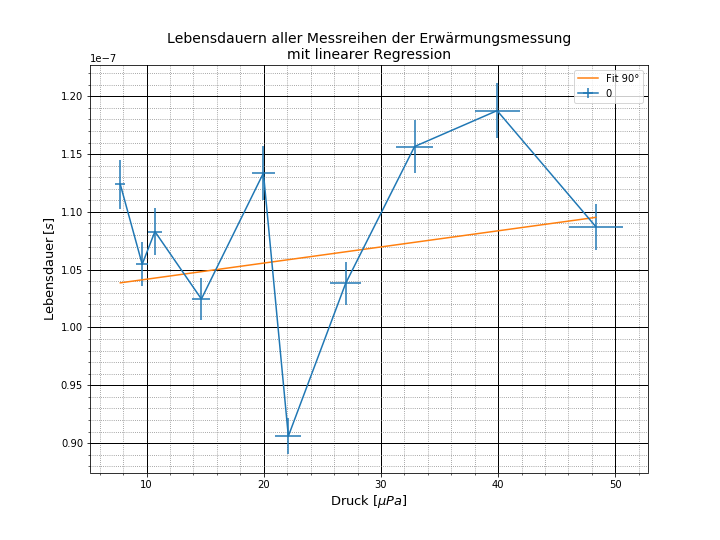
\includegraphics[scale=0.5]{Bild/Auf}
	\centering
	\caption[Druck zu Lebensdauer Fit für Aufwärmung]{Aufwärmmessung der ersten Messreihe für $0^\circ$. Die Datenpunkte sind mit Fehlern für Lebensdauer und Druck aber für den Fit wurden nur die dominanteren der Lebensdauer verwendet.}
	\label{Auf1}
\end{figure}
\FloatBarrier
\subsubsection{Lebensdauern der Abkühlmessung 2}
Für die zweite Abkühlungsmessung ergeben die nachfolgenden Parameter aus den Angepassten Kurven in Fig. \ref{Abk2}:
\begin{equation*}
f(p)_{0^\circ}=(8.2\pm 2.7)\cdot 10^{-11} \frac{\text{s}}{\text{$\mu$Pa}}\cdot p + (1.166\pm 0.017)\cdot 10^{-7} \text{s}
\end{equation*}
\begin{equation*}
f(p)_{90^\circ}=(1.7\pm 0.5)\cdot 10^{-11} \frac{\text{s}}{\text{$\mu$Pa}}\cdot p + (1.181\pm 0.018)\cdot 10^{-7} \text{s}
\end{equation*}
Hierbei ist der y-Achsen Abschnitt jeweils die gesuchte Lebensdauer.
\begin{figure}[ht]
	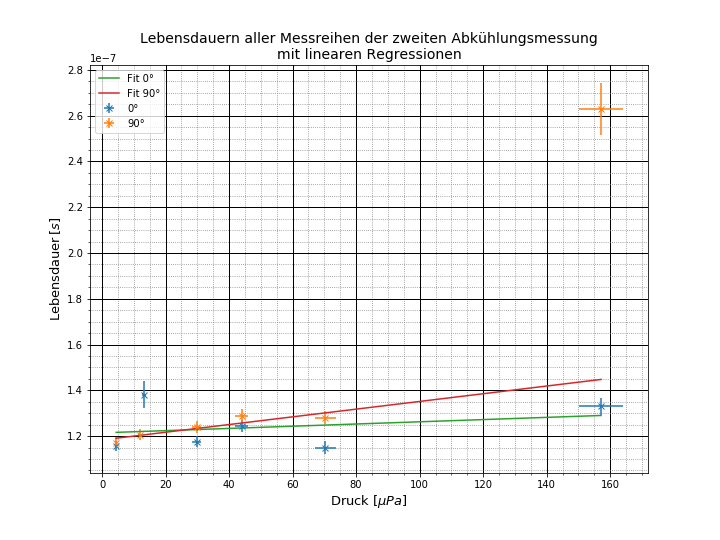
\includegraphics[scale=0.5]{Bild/Abk2}
	\centering
	\caption[Druck zu Lebensdauer Fit für Abkühlung 2]{Abkühlungsmessung der zweiten Messreihe einmal für $90^\circ$ und einmal für $0^\circ$. Die Datenpunkte sind mit Fehlern für Lebensdauer und Druck aber für den Fit wurden nur die dominanteren der Lebensdauer verwendet. Der Messpunkt bei ca. $160\,\mu$Pa der 90$^\circ$ Messreihe wurde als Ausreißer nicht mit zur Regression verwendet.}
	\label{Abk2}
\end{figure}
\FloatBarrier
\subsection{Messungen zu 45$^\circ$}
Ursprünglicher weise wurden mehrere Messungen bei einem Winkel von $45^\circ$ durchgeführt. Jedoch gelang es weder die Ableitung von Formel \ref{Lorenzfit} nach x (vgl. Fig. \ref{45deg}) noch die Formel \ref{EasyFit} ausreichend bzw. generell zu fitten. Dies lag besonders an der unsymmetrischen Form der Messreihe.
\begin{figure}[ht]
	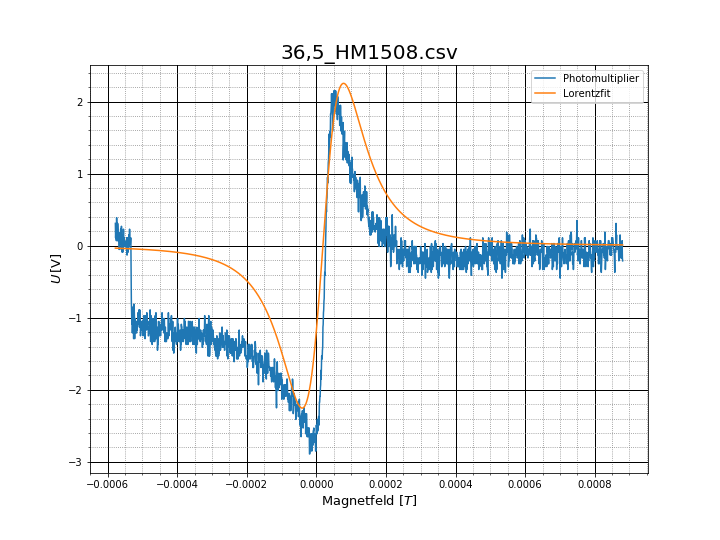
\includegraphics[scale=0.5]{Bild/45_fit}
	\centering
	\caption[Druck zu Lebensdauer Fit für eine Beliebige 45$\circ$ Messung]{Die Daten der ersten 45$^\circ$ Messung der ersten Abkühlungsmessreihe mit dem Fit nach der Ableitung von Formel \ref{Lorenzfit}. Es ist sichtbar, dass die gefittete Funktion den Daten ähnelt, jedoch die Parameter nicht hinreichend optimiert wurden konnten um quantitative Aussagen treffen zu können.}
	\label{45deg}
\end{figure}